%% 30min talk

\documentclass[english]{beamer}
\usetheme{Warsaw}
\setbeamertemplate{navigation symbols}{} % remove the navigation symbols
\setbeamertemplate{headline}{} % remove headline
\setbeamertemplate{footline}[frame number]

\usepackage{babel}
\usepackage[utf8]{inputenc}
\usepackage{textcomp}
\usepackage{wasysym}

\title{Beyond-the-standard-model contributions to rare B decays analyzed with variational-Bayes enhanced adaptive importance sampling}
\author{Stephan Jahn}
\date{\today} %TODO: insert date

% ----------------------------------------------------------------------

\begin{document}

\newcommand{\slide}[2][t]{\begin{frame}[#1] \frametitle{\insertsection} #2 \end{frame}}

% ----------------------- title page, unnumbered -----------------------

{
\setbeamertemplate{footline}{}
\frame[nopagenumbering]{\titlepage}
}

% -------------------------- overview section --------------------------

\section{Overview}

\slide[t]{

    Bayes' formula:
    \newline \newline
    $$ P(\theta | \mathcal{D}, \mathrm{M} ) = \frac{P(\mathcal{D}|\theta, \mathrm{M})P(\theta | \mathrm{M})}{P(\mathcal{D} | \mathrm{M} )}
       = \frac{P(\mathcal{D}|\theta, \mathrm{M})P(\theta | \mathrm{M})}{\int P(\mathcal{D}|\theta, \mathrm{M})P(\theta | \mathrm{M}) d\theta }$$

    \only<2->{ \
        \newline \newline \
        our application: \
        \
        \newline \newline \

        \only<3->{$$ \theta = \lbrace \mathcal{C}_{7 , 9 , 10 , S , P , T , T5 , ...}^{(\prime)} \rbrace $$}
        \only<4->{$$ \mathcal{D} = \mathrm{experimental~data} $$}
        \only<5->{$$ \mathrm{M} = \mathrm{EFT , SM , ...} $$}
    }

}


\slide[t]{

{\large\textbf{Goals}}

\begin{columns}[t] % The "c" option specifies centered vertical alignment while the "t" option is used for top vertical alignment

\column{.45\textwidth} % Left column and width

\only<2->{\begin{itemize}
              \item draw marginal plots of the posterior
              \
              \newline

              \hspace{-1.2cm} 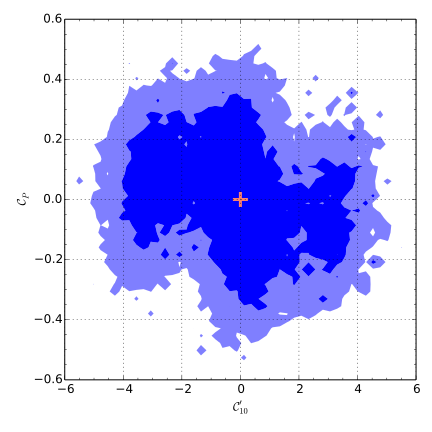
\includegraphics[width=1.01\textwidth]{figures/C10p_CP}

          \end{itemize}}

\column{.5\textwidth} % Right column and width

\only<3->{\begin{itemize}
          \item compare models $\mathrm{EFT} \leftrightarrow \mathrm{SM}$
          \end{itemize}

              $$ \frac{P(\mathrm{EFT}|\mathcal{D})}{P(\mathrm{SM}|\mathcal{D})} =
                 \frac{P(\mathcal{D}|\mathrm{EFT})}{P(\mathcal{D}|\mathrm{SM})} \cdot \frac{P(\mathrm{EFT})}{P(\mathrm{SM})} $$

              $$ P(\mathrm{M} | \mathcal{D} ) = \frac{P(\mathcal{D} | \mathrm{M})P(\mathrm{M})}{P(\mathcal{D})} $$

          \begin{itemize}
          \item[]
              \begin{itemize}
                  \item[] \only<4->{\hspace{-0.1\textwidth} $\frac{P(\mathrm{EFT}|\mathcal{D})}{P(\mathrm{SM}|\mathcal{D})} > 1$ new physics \smiley{} \newline}
                  \item[] \only<5->{\hspace{-0.1\textwidth} $\frac{P(\mathrm{EFT}|\mathcal{D})}{P(\mathrm{SM}|\mathcal{D})} < 1$ confirm SM \frownie{}}
              \end{itemize}
          \end{itemize}}

\end{columns}

}





\slide[t]{

{\large\textbf{Difficulties}}

\begin{columns}[t] % The "c" option specifies centered vertical alignment while the "t" option is used for top vertical alignment

\column{.45\textwidth} % Left column and width

\vspace{0.65cm} % to center the text

\only<2->{\begin{itemize}}
\only<2->{\item curse of dimensionality}
\only<3->{\item multimodality}
\only<4->{\item degeneracies}
\only<2->{\end{itemize}}

\only<5->{\Huge \textcolor{red}{no standard algorithm so far}}

\column{.5\textwidth} % Right column and width

\vspace{-8mm}

\begin{center}
\only<3->{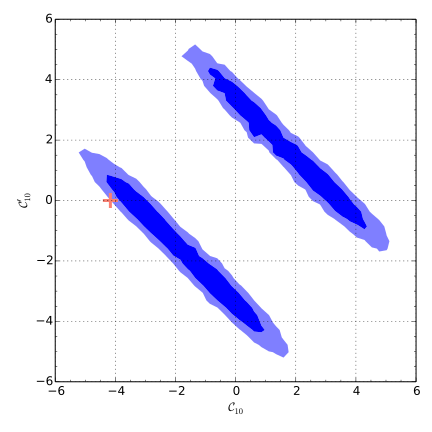
\includegraphics[height=0.4\textheight]{figures/C10_C10p}}

\only<4->{\includegraphics[height=0.43\textheight]{figures/example_for_degeneracy}}
\end{center}


\end{columns}

}

% ------------------------------ toc page ------------------------------

\begin{frame}
\frametitle{Contents}
\tableofcontents
\end{frame}

% ----------------------------- VB section -----------------------------

\section{Adaptive importance sampling with the variational-Bayes approach} %TODO: write

%TODO: mention pypmc in detail; that is a major outcome of the work

\slide{ %TODO: remove or modify this slide

    \textlangle empty\textrangle

}

\subsection{Adaptive importance sampling}

\slide{ %TODO: remove or modify this slide

    \frametitle{\insertsubsectionhead}

    \only<1-2> {placeholder 1}
    \only<2> {placeholder 2}
    \only<-3> {placeholder 3}
    \only<4> {placeholder 4}

}

\subsection{Variational Bayes}

\slide{ %TODO: remove or modify this slide

    \frametitle{\insertsubsectionhead}

    \only<1-2> {placeholder 1}
    \only<2> {placeholder 2}
    \only<-3> {placeholder 3}
    \only<4> {placeholder 4}

}

% ------------------------- B-physics section --------------------------

\section{Scalar and tensor contributions to $ b \to s \mu^+ \mu^- $} %TODO: write

\slide{ %TODO: remove or modify this slide

    \textlangle empty\textrangle

}

\subsection{scalar contributions}

\slide{ %TODO: remove or modify this slide

    \frametitle{\insertsubsectionhead}

    \only<1-2> {placeholder 1}
    \only<2> {placeholder 2}
    \only<-3> {placeholder 3}
    \only<4> {placeholder 4}

}

\subsection{tensor contributions}

\slide{ %TODO: remove or modify this slide

    \frametitle{\insertsubsectionhead}

    \only<1-2> {placeholder 1}
    \only<2> {placeholder 2}
    \only<-3> {placeholder 3}
    \only<4> {placeholder 4}

}

\end{document}
